\documentclass[red]{beamer}

\usetheme{default}
%\usetheme{CambridgeUS}
%\usetheme{Frankfurt}

% Uncomment the following line if you want %
% page numbers and using Warsaw theme%
%\setbeamertemplate{footline}[page number]
%\setbeamercovered{transparent}
%\setbeamercovered{invisible}

% To remove the navigation symbols from 
% the bottom of slides%
\setbeamertemplate{navigation symbols}{} 

\usepackage{amsfonts}
\usepackage{amsmath}
\usepackage{amsthm}
\usepackage{amssymb}
\usepackage{graphicx}

\usepackage[american]{babel}
\usepackage{csquotes}
\usepackage[style=apa,natbib=true,backend=biber]{biblatex}
\DeclareLanguageMapping{american}{american-apa}
\addbibresource{Polarization.bib}

\usepackage{hyperref}
\ExecuteBibliographyOptions{doi=false}
\newbibmacro{string+doi}[1]{%
  \iffieldundef{doi}{#1}{\href{http://dx.doi.org/\thefield{doi}}{#1}}}
\DeclareFieldFormat{title}{\usebibmacro{string+doi}{\mkbibemph{#1}}}
\DeclareFieldFormat[article]{title}{\usebibmacro{string+doi}{\mkbibquote{#1}}}

%\usepackage{bm}         % For typesetting bold math (not \mathbold)

%\logo{\includegraphics[height=0.6cm]{yourlogo.eps}}
%

\title[Polarization and Tasks]{Tasks and Work Force Polarization}
\author{Alex Cooper}
\institute[Macquarie University]
{ Honors Candidate \\ Macquarie University \\
\medskip
{\emph{alexander.cooper@students.mq.edu.au}}
}
\date{7 June 2013}
\begin{document}
%
\begin{frame}
\titlepage
\end{frame}
%
\section{International Experience}
\subsection{}

\begin{frame}[t]{United States}
\frametitle{Wage inequality has risen since 1960s}
\begin{center}
  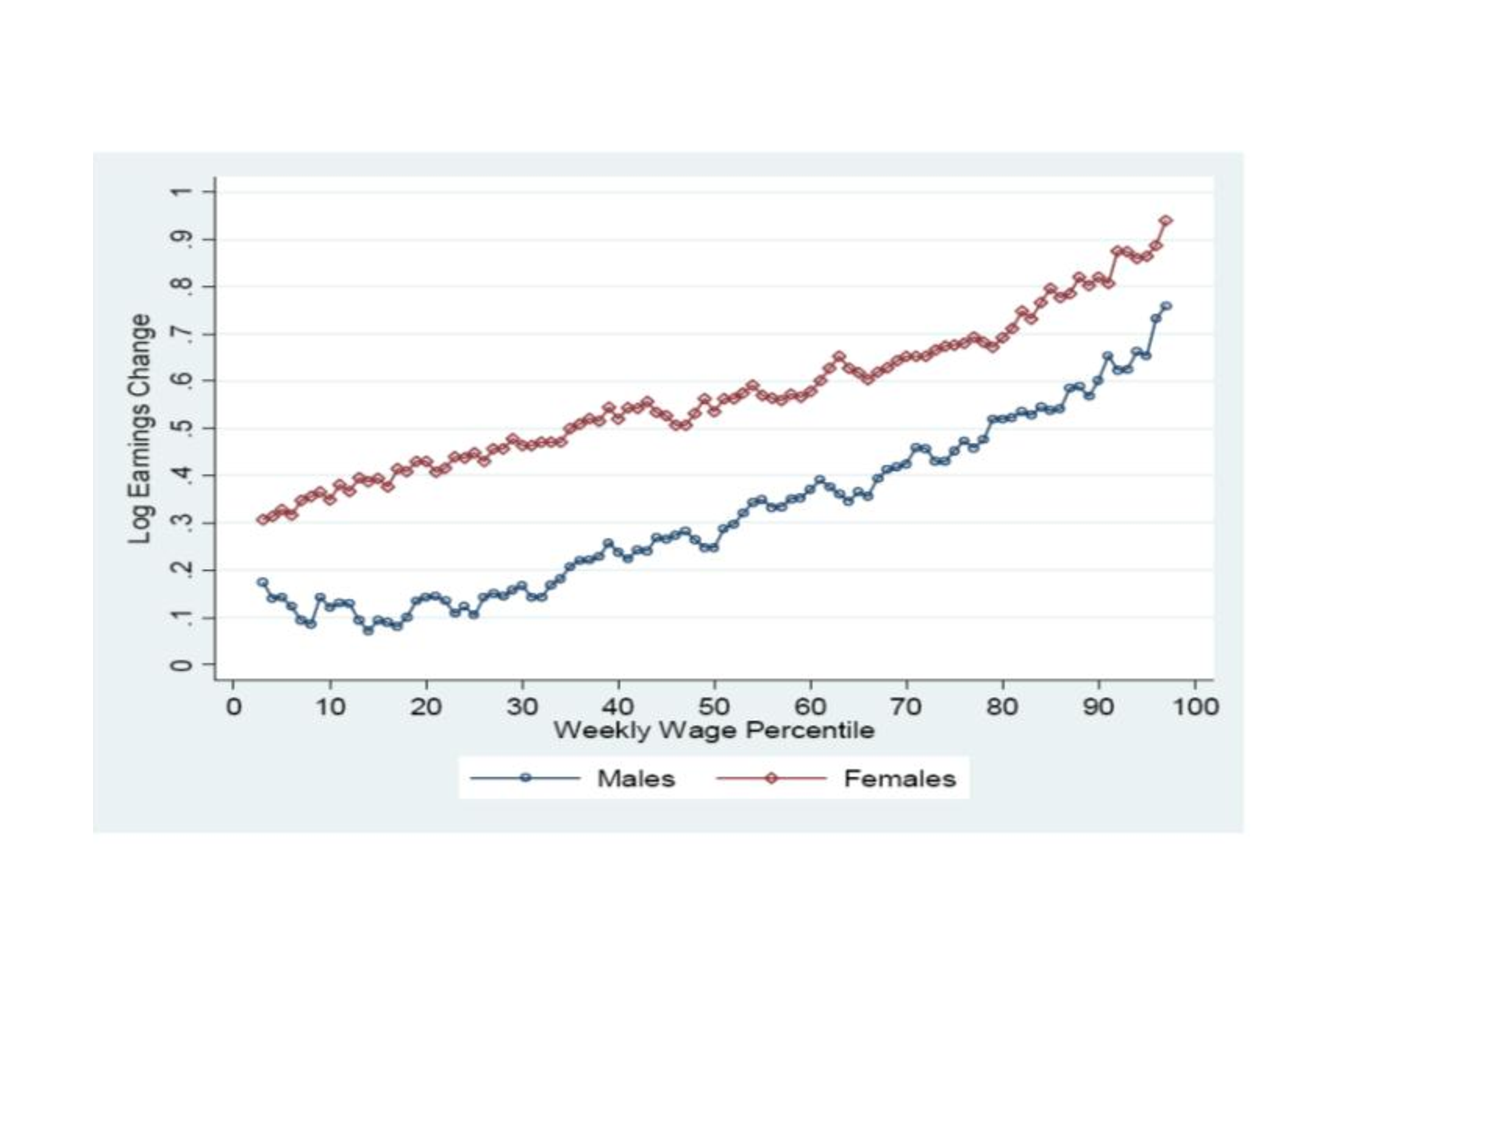
\includegraphics[width=\textwidth]{slides/katz_kearney_2008_log_e_chg.pdf}
  \\
  Change in Log Real Weekly Wage by Perecntile, Full-Time Workers, 1963-2005.
  \citep{Autor2008}
\end{center}
\end{frame}

\begin{frame}
\frametitle{Skill-Based Technical Change (SBTC)}
\begin{itemize}
\item Model features:
\begin{itemize}
\item Two skills, high ($H$) and low ($L$).
\item $H$ and $L$ are different, and imperfect productive substitutes: $\sigma>0$.
\item Technology \emph{factor-augmenting}: always raises productivity/wages.
\item Wages set on the demand curve
\end{itemize}
\item Empirically successful. e.g.
  \begin{itemize}
  \item \cite{Katz1992}
  \item \cite{CardLemieux2001}
  \end{itemize}
\end{itemize}
\end{frame}

\begin{frame}
\frametitle{The `Canonical Model' of Skill-Based Technical Change}
\begin{itemize}
\item Production function representation:
\begin{equation}
  \label{eq:cobbdoug}
  F(L,H) = \left[\left(A_LL\right)^{\frac{\sigma - 1}{\sigma}}
            + \left(A_HH\right)^{\frac{\sigma - 1}{\sigma}}
          \right]^\frac{\sigma}{(\sigma-1)}
\end{equation}
\item Empirical implications depend on $\sigma$. SBTC implies
  \begin{itemize}
  \item Rise in $A_H/A_L$ if $H$ and $L$ are gross substitutes ($\sigma > 1$)
  \item Fall in $A_H/A_L$ if $H$ and $L$ are gross complements ($\sigma > 1$)
  \end{itemize}
\item Predicts
  \begin{itemize}
  \item Increasing inequality, driven by skill demand.
  \item Rising college/education premium.
  \item Monotone wage growth in skills.
  \end{itemize}
\end{itemize}
\end{frame}

\begin{frame}[t]{United States}
\frametitle{Non-monotone increases in wage by skill percentile (USA)}
\begin{center}
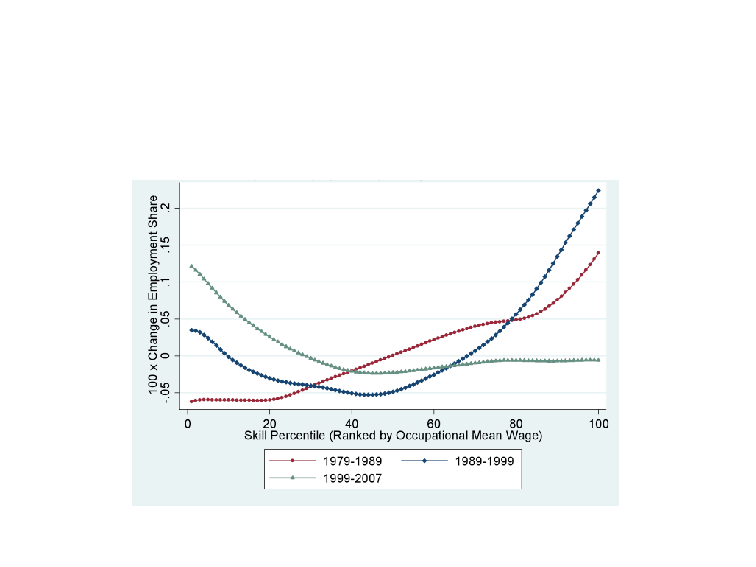
\includegraphics[width=\textwidth]{slides/emp_occ_skill_percentile.pdf}
\\
Smoothed changes in employment by occupational skill percentile, 1979-2007
\citep{Acemoglu2011}
\end{center}
\end{frame}

\section{Alternative Model}
\begin{frame}[fragile] % Notice the [fragile] option %
\frametitle{\cite{Levy2003}}
``The skill content of recent technological change: An empirical exploration.'' \emph{The Quarterly Journal of Economics}, 118(4), 1279--1333.

\begin{itemize}
\item Jobs have different \emph{task content}, so technology can be factor-augmenting or a substitute.
\item Two kinds of labor: routine ($L_R$), and non-routine ($L_N$). Capital is perfectly substitutable for non-routine tasks:
$$ F(R,N) = (L_R + C)^{1-\beta}L_N^{\beta},\quad\beta\in(0,1)$$
\item Workers are endowed with a fixed set of skills, inelastically supply 1 unit of labor.
\item `Ricardian' model: assignment of workers to tasks is endogenous (as in \cite{Roy1951}).
\end{itemize}
\end{frame}

\begin{frame}
  \frametitle{Job Polarization: United States}
  \begin{center}
  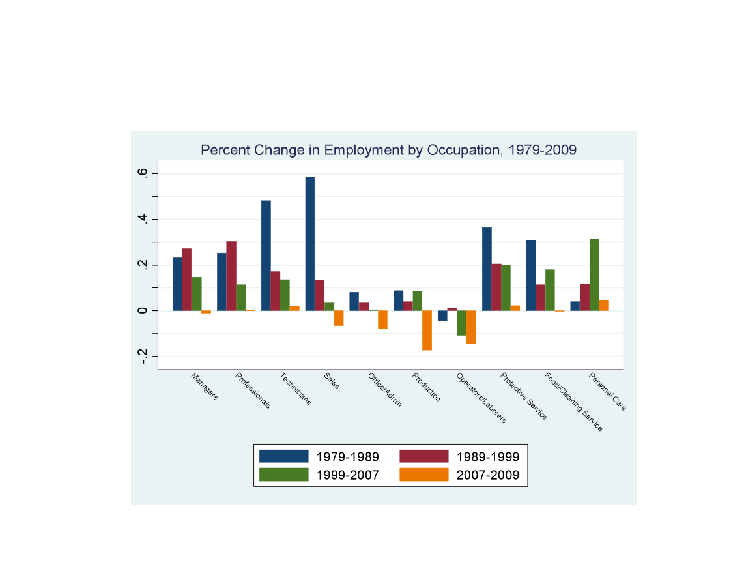
\includegraphics[width=0.9\textwidth]{slides/level_by_occ.pdf} \\
  Percentage change in employment level, by occupation group, USA, 1979-2009 \citep{Acemoglu2011}
  \end{center}
\end{frame}

\begin{frame}
  \frametitle{This Project}
  \begin{enumerate}
  \item  Has employment in Australia polarized in terms of routine and non-routine tasks as it has overseas?
    \begin{itemize}
    \item If not, why is Australia special?
    \end{itemize}
  \item Does ICT capital investment explain this trend?
  \end{enumerate}
\end{frame}

\begin{frame}
  \frametitle{Data}
  \begin{enumerate}
  \item O*NET: Occupational task database
    \begin{itemize}
    \item Developed by US Department of Commerce
    \item Detailed break-down of activities, skills and abilities by occupation
    \end{itemize}
  \item Australian Bureau of Statistics
    \begin{itemize}
    \item Labor Force Survey (LFS)
    \item Survey of Income and Housing
    \item Census of Population and Housing
    \item National accounts: ICT and Machinery investment, capital stock
    \end{itemize}
  \end{enumerate}
\end{frame}

\begin{frame}
  \begin{center}
    Questions?    
  \end{center}
\end{frame}

\begin{frame}
\frametitle{References}
\printbibliography
\end{frame}

\begin{frame}
  \begin{center}
    Spare Slides
  \end{center}
\end{frame}

\begin{frame}
\frametitle{O*NET Data Example}
\begin{table}[htbp]
\begin{tabular}{|p{2cm}|p{1.65cm}|p{1.5cm}|p{1.5cm}|p{1.5cm}|}
\hline
{Job Title} & {Get Data} & {Analyze Data} & {\small Think Creatively} & {Handle Moving Objects} \\ \hline
{CEOs} & 5.03 & 4.82 & 5.1 & 1.1  \\ \hline
{Economists} & 5.88 & 6.58 & 5.38 & 0.54 \\ \hline
{Dancers} & 3.88 & 1.96 & 4.37 & 2.63 \\ \hline
{Programmers} & 4.91 & 5.05 & 5.96 & 0.44 \\ \hline
{Tellers} & 2.91 & 2.65 & 2.21 & 2.74 \\ \hline
{Surgeons} & 5.72 & 5.49 & 4.67 & 3.62 \\ \hline
{Bakers} & 2.8 & 3.29 & 2.93 & 5.06 \\ \hline
{Receptionists} & 3.1 & 2.45 & 2.54 & 2.88 \\ \hline
{Typists} & 4.35 & 1.52 & 3.9 & 1.43 \\ \hline
\end{tabular}
\caption{O*NET Work Activity Example (Levels, Scale 0--7)}
\label{onetex}
\end{table}
\end{frame}

\end{document} 
